\documentclass{article}%
\usepackage{amsmath}
\usepackage{amsfonts}
\usepackage{amssymb}
\usepackage{graphicx}
\usepackage{tikz}
\usepackage{hyperref}%
\setcounter{MaxMatrixCols}{30}
%TCIDATA{OutputFilter=latex2.dll}
%TCIDATA{Version=5.00.0.2552}
%TCIDATA{CSTFile=40 LaTeX article.cst}
%TCIDATA{Created=Thursday, August 21, 2008 14:03:59}
%TCIDATA{LastRevised=Wednesday, October 01, 2014 12:46:33}
%TCIDATA{<META NAME="GraphicsSave" CONTENT="32">}
%TCIDATA{<META NAME="SaveForMode" CONTENT="1">}
%TCIDATA{<META NAME="DocumentShell" CONTENT="Standard LaTeX\Blank - Standard LaTeX Article">}
%TCIDATA{Language=American English}
\newtheorem{theorem}{Theorem}
\newtheorem{acknowledgement}[theorem]{Acknowledgement}
\newtheorem{algorithm}[theorem]{Algorithm}
\newtheorem{axiom}[theorem]{Axiom}
\newtheorem{case}[theorem]{Case}
\newtheorem{claim}[theorem]{Claim}
\newtheorem{conclusion}[theorem]{Conclusion}
\newtheorem{condition}[theorem]{Condition}
\newtheorem{conjecture}[theorem]{Conjecture}
\newtheorem{corollary}[theorem]{Corollary}
\newtheorem{criterion}[theorem]{Criterion}
\newtheorem{definition}[theorem]{Definition}
\newtheorem{example}[theorem]{Example}
\newtheorem{exercise}[theorem]{Exercise}
\newtheorem{lemma}[theorem]{Lemma}
\newtheorem{notation}[theorem]{Notation}
\newtheorem{problem}[theorem]{Problem}
\newtheorem{proposition}[theorem]{Proposition}
\newtheorem{remark}[theorem]{Remark}
\newtheorem{solution}[theorem]{Solution}
\newtheorem{summary}[theorem]{Summary}
\newenvironment{proof}[1][Proof]{\noindent\textbf{#1.} }{\ \rule{0.5em}{0.5em}}
\begin{document}

\title{Graph Theory Final}
\author{Christopher Chapline}
\maketitle
\section{Problem 1}

\subsection{$C_5$}

% Draw the cycle on 5 vertices
\begin{tikzpicture}
    \tikzstyle{vertex}=[draw=black!25,shape=circle, edge=black!25,minimum size=20pt,inner sep=0pt]

    \def \n {4}
    \def \radius {3cm}
    \def \margin {8} % margin in angles, depends on the radius

    \foreach \s in {1,...,\n}
    {
        \node[vertex] at ({360/\n * (\s - 1)}:\radius) {$\s$};
        \draw[-, >=latex] ({360/\n * (\s - 1)+\margin}:\radius)
            arc ({360/\n * (\s - 1)+\margin}:{360/\n * (\s)-\margin}:\radius);
    }
\end{tikzpicture}

This graph is:
\begin{itemize}
    \item Planar (it is drawn above)
    \item Eulerian (Every vertex is even and it is connected)
    \item Hamiltonian (Every cycle graph is Hamiltonian)
    \item NOT traversible (No odd vertices)
\end{itemize}

\subsection{$C_{20}$}
% Draw the cycle on 20 vertices
\begin{tikzpicture}
    \tikzstyle{vertex}=[draw=black!25,shape=circle, edge=black!25,minimum size=20pt,inner sep=0pt]

    \def \n {20}
    \def \radius {3cm}
    \def \margin {8} % margin in angles, depends on the radius

    \foreach \s in {1,...,\n}
    {
        \node[vertex] at ({360/\n * (\s - 1)}:\radius) {$\s$};
        \draw[-, >=latex] ({360/\n * (\s - 1)+\margin}:\radius)
            arc ({360/\n * (\s - 1)+\margin}:{360/\n * (\s)-\margin}:\radius);
    }
\end{tikzpicture}

This graph is:
\begin{itemize}
    \item Planar (it is drawn above)
    \item Eulerian (Every vertex is even and it is connected)
    \item Hamiltonian (Every cycle graph is Hamiltonian)
    \item NOT traversible (No odd vertices)
\end{itemize}

\subsection{$P_5$}
\begin{tikzpicture}
    \tikzstyle{vertex}=[draw=black!25,shape=circle, edge=black!25,minimum size=20pt,inner sep=0pt]

    \node[vertex] (1) at (2,0) {1};
    \node[vertex] (2) at (4,0) {2};
    \node[vertex] (3) at (6,0) {3};
    \node[vertex] (4) at (8,0) {4};
    \node[vertex] (5) at (10,0) {5};

    \draw (1) -- (2) -- (3) -- (4) -- (5);
\end{tikzpicture}

This graph is:
\begin{itemize}
    \item Planar (it is drawn above)
    \item NOT Eulerian (It has odd vertices)
    \item Hamiltonian (Every cycle graph is Hamiltonian)
    \item NOT traversible (No odd vertices)
\end{itemize}

\subsection{$K_4$}

\begin{tikzpicture}
    \tikzstyle{vertex}=[draw=black!25,shape=circle, edge=black!25,minimum size=20pt,inner sep=0pt]

    \node[vertex] (1) at (2,0) {1};
    \node[vertex] (2) at (0,2) {2};
    \node[vertex] (3) at (-2,0) {3};
    \node[vertex] (4) at (0,-2) {4};

    \draw (4) -- (1) -- (2) -- (3) -- (4) -- (2);
    \draw (3) to [bend left] (0, 3) to [bend left] (1);
\end{tikzpicture}

This graph is:
\begin{itemize}
    \item Planar (it is drawn above)
    \item NOT Eulerian (It has odd vertices)
    \item Hamiltonian (Every complete graph is Hamiltonian)
    \item NOT traversible (Every vertex is degree 3)
\end{itemize}

\subsection{$K_{3, 4}$}

\begin{tikzpicture}
    \tikzstyle{vertex}=[draw=black!25,shape=circle, edge=black!25,minimum size=20pt,inner sep=0pt]

    \node[vertex, fill=blue!25] (a) at (1,1) {a};
    \node[vertex, fill=blue!25] (b) at (1,3) {b};
    \node[vertex, fill=blue!25] (c) at (1,5) {c};

    \node[vertex, fill=red!25] (1) at (10,0) {1};
    \node[vertex, fill=red!25] (2) at (10,2) {2};
    \node[vertex, fill=red!25] (3) at (10,4) {3};
    \node[vertex, fill=red!25] (4) at (10,6) {4};

    \draw (a) -- (1);
    \draw (a) -- (2);
    \draw (a) -- (3);
    \draw (a) -- (4);

    \draw (b) -- (1);
    \draw (b) -- (2);
    \draw (b) -- (3);
    \draw (b) -- (4);

    \draw (c) -- (1);
    \draw (c) -- (2);
    \draw (c) -- (3);
    \draw (c) -- (4);
\end{tikzpicture}

This graph is:
\begin{itemize}
    \item NOT Planar (Subgraph isomorphic to $K_{3,3}$)
    \item NOT Eulerian (It has odd vertices)
    \item NOT Hamiltonian
    \item NOT traversible (4 vertices degree 3)
\end{itemize}

\section{Problem 2}

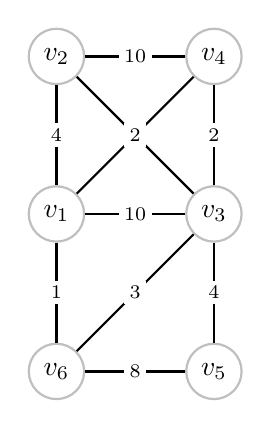
\begin{tikzpicture}
    \tikzstyle{vertex}=[draw=black!25,shape=circle, edge=black!25,minimum size=20pt,inner sep=0pt]
    \tikzstyle{edge} = [draw,thick,-]
    \tikzstyle{arrow} =[draw,thick,->]
    \tikzstyle{weight} = [draw=none,fill=white,inner sep=2pt,font=\scriptsize]

    \node[vertex] (1) at (0, 2) {$v_1$};
    \node[vertex] (2) at (0, 4) {$v_2$};
    \node[vertex] (3) at (2, 2) {$v_3$};
    \node[vertex] (4) at (2, 4) {$v_4$};
    \node[vertex] (5) at (2, 0) {$v_5$};
    \node[vertex] (6) at (0, 0) {$v_6$};

    \path[edge] (2) -- node[weight] {10} (4);
    \path[edge] (2) -- node[weight] {4} (1);
    \path[edge] (2) -- node[weight] {9} (3);
    \path[edge] (1) -- node[weight] {1} (6);
    \path[edge] (1) -- node[weight] {10} (3);
    \path[edge] (1) -- node[weight] {2} (4);
    \path[edge] (3) -- node[weight] {2} (4);
    \path[edge] (3) -- node[weight] {4} (5);
    \path[edge] (3) -- node[weight] {3} (6);
    \path[edge] (6) -- node[weight] {8} (5);
\end{tikzpicture}

\subsection{Part A}
\subsection{Part B}
\subsection{Part C}

\section{Problem 3}

\subsection{Part A}

Let's first calculate the vertex set for $K_2 \times K_2$.\\ \\
$V(K_2 \times K_2) = V(K_2) \times V(K_2) = \{1, 2\} \times \{1, 2\} = \{(1, 1), (1, 2), (2, 1), (2, 2)\}$ \\ \\
Let's now determine which edges will be present in our graph:
\begin{itemize}
    \item There will be an edge between $(1, 1)$ and $(1, 2)$ because $1 \in V(K_2)$ and $(1,2) \in E(K_2)$
    \item There will be an edge between $(2, 1)$ and $(2, 2)$ because $2 \in V(K_2)$ and $(1,2) \in E(K_2)$
    \item There will be an edge between $(1, 2)$ and $(2, 2)$ because $2 \in V(K_2)$ and $(1,2) \in E(K_2)$
    \item There will be an edge between $(2, 1)$ and $(1, 1)$ because $1 \in V(K_2)$ and $(1,2) \in E(V_2)$
\end{itemize}

A drawing of the resultant graph follows:

\begin{tikzpicture}
    \tikzstyle{vertex}=[draw=black!25,shape=circle, edge=black!25,minimum size=20pt,inner sep=0pt]

    \node[vertex] (1) at (-1, -1) {$(1,1)$};
    \node[vertex] (2) at (-1, 1) {$(1,2)$};
    \node[vertex] (3) at (1, -1) {$(2,1)$};
    \node[vertex] (4) at (1, 1) {$(2,2)$};

    \draw (1) -- (2) -- (4) -- (3) -- (1)
\end{tikzpicture} \\

The graph of $C_4$ is also shown below:

\begin{tikzpicture}
    \tikzstyle{vertex}=[draw=black!25,shape=circle, edge=black!25,minimum size=20pt,inner sep=0pt]

    \node[vertex] (1) at (-1, -1) {$1$};
    \node[vertex] (2) at (-1, 1) {$2$};
    \node[vertex] (3) at (1, -1) {$3$};
    \node[vertex] (4) at (1, 1) {$4$};

    \draw (1) -- (2) -- (4) -- (3) -- (1)
\end{tikzpicture} \\

We can define a mapping function between $C_4$ and $K_2$ to show that they are isomorphic:\\
 \begin{displaymath}
   \varphi(v) = \left\{
     \begin{array}{lr}
         (1, 1) & :v = 1 \\
         (1, 2) & :v = 2 \\
         (2, 2) & :v = 3 \\
         (2, 1) & :v = 4
     \end{array}
   \right.
\end{displaymath}

\subsection{Part B}
\begin{theorem}
    There are $2^n$ vertices and $n2^{n-1}$ edges in $Q_n$.
\end{theorem}

\begin{proof}
    We will induct on $n$\\ \\
    We will establish $n=1$ as our base case. $Q_1$ is defined as being $K_2$, which has two vertices and a single edge. In this case:

    $2^1 = 2$ \checkmark

    $(1)2^0 = 1$ \checkmark \\ \\
    For the inductive case, we will assume that $Q_n$ has $2^n$ vertices and $n2^{n-1}$ edges and we must show that $Q_{n+1}$ has $2^{n+1}$ vertices and $(n+1)2^n$ edges. We know that $Q_{n+1} = K_2 \times Q_n$. The cartesian product between $K_2$ and $Q_n$ will have a vertex set equal to $V(Q_n) \times V(K_2)$. This set will have all of the elements from $V(Q_n)$ two separate times (once for each element in $V(K_2)$, yielding a final vertex set with $2^{n+1}$ elements. We know that there are $n2^{n-1}$ edges in $Q_n$. The number of edges present in $Q_{n+1}$ will be equal to the number of edges in $Q_n$ multiplied by $n + 1$, which is the current

    Therefore, the hypercube $Q_{n+1}$ will have $2^{n+1}$ vertices and $(n+1)2^n$ edges.
\end{proof}

\subsection{Part C}

$E \geq 2F$ \\
$V + F + 2 -2g \geq 4 - 4g + 2E - V$ \\
$6g \geq 2 - V - F + 2E - V$ \\
$6g \geq 2 + 2E - 2V - F$ \\
$4g \geq n2^{n-1} - 2^n$ \\
$g \geq n2^{n-3} - 2^{n-2}$ \\ \\
Couldn't quite get there.

\section{Problem 5}
\subsection{Part A}
\begin{theorem}
$B_1$ is matched with $B_2$
\end{theorem}

\begin{proof}
    Assume that $B_1$ is not matched with $G_1$, but is instead matched with some girl $G_i$ where $i \neq 1$. This would imply that $G_1$ is matched with some boy $B_j$ where $j \neq 1$. This matching produces an unstable marriage because $B_1$ prefers $G_1$ more than he prefers $G_i$ and $G_1$ prefers $B_1$ more than she prefers $B_j$. \\ \\
    Therefore, $B_1$ must be matched with $G_1$.
\end{proof}

\subsection{Part B}
\begin{theorem}
$B_n$ is matched with $G_n$, $\forall n$.
\end{theorem}

\begin{proof}
We will induct on $n$.\\ \\
In the case where $n=1$, we know that $B_1$ is matched with $G_1$ because they are the only matching possible and therefore must produce a stable marriage. \\ \\
Otherwise, we assume that $B_n$ is matched $G_n$. We must show that $B_{n+1}$ must be matched with $G_{n+1}$. Assume that $B_{n+1}$ is instead matched with some girl $G_i$ where $i > (n+1)$ and assume that $G_{n+1}$ is matched with some boy $B_j$ where $j > (n+1)$. Observe that $G_{n+1}$ prefers $B_{n+1}$ more than she prefers $B_j$. Furthermore, observe that $B_{n+1}$ prefers $G_{n+1}$ more than he prefers $G_i$. Because $B_{n+1}$ and $G_{n+1}$ prefer each other more than they prefer their matched spouses, they are a rogue couple. This means that $B_{n+1}$ must be matched with $G_{n+1}$.\\ \\
    Therefore, $B_n$ is matched with $G_n$, $\forall n$.

\end{proof}

\subsection{Part C}
\begin{theorem}
The mating ritual will find a stable marriage in one day
\end{theorem}

\begin{proof}
    On the first day, every boy will go to the girl that they prefer the most. Since every boy $B_i$ prefers $G_i$ as their top pick, each boy will go to a different girl. Regardless of the girl's preferences, the mating ritual will end since every girl was only presented with a single boy to choose. \\ \\
    Therefore, the mating ritual will only last a single day.
\end{proof}

\section{Problem 6}
She can increase the ranking of the pages that she desires by multiplying by a scalar value $\omega \leq (n_j - 1)$. To normalize the rankings, she must then divide all other columns by $\frac{\omega}{n_j - 1}$. This will ensure that the additive matrix $S$ remains column stochastic and ensures that the rankings are well-defined on the web. If she wishes to increase the rankings for multiple pages, then she must perform a similar procedure, although she must ensure that the matrix remains column stochastic throughout the tampering process, otherwise she risks ending up with a matrix that is not well-defined. Under a probabilistic interpretation of PageRank, this will increase the probability that you will randomly jump to one of the desired pages, while simultaneously decreasing the probability that you'll jump to one of the less-desirable pages.
\end{document}
